\documentclass[letterpaper]{article}
\usepackage[margin=1in]{geometry}
\usepackage[utf8]{inputenc}
\usepackage{textcomp}
\usepackage{amssymb}
\usepackage{natbib}
\usepackage{graphicx}
\usepackage{gensymb}
\usepackage{amsthm, amsmath, mathtools}
\usepackage[dvipsnames]{xcolor}
\usepackage{enumerate}
\usepackage{mdframed}
\usepackage[most]{tcolorbox}
\usepackage{csquotes}
% https://tex.stackexchange.com/questions/13506/how-to-continue-the-framed-text-box-on-multiple-pages

\tcbuselibrary{theorems}

\newcommand{\R}{\mathbb{R}}
\newcommand{\Z}{\mathbb{Z}}
\newcommand{\N}{\mathbb{N}}
\newcommand{\Q}{\mathbb{Q}}
\newcommand{\C}{\mathbb{C}}
\newcommand{\code}[1]{\texttt{#1}}
\newcommand{\mdiamond}{$\diamondsuit$}
\newcommand{\PowerSet}{\mathcal{P}}
\newcommand{\Mod}[1]{\ (\mathrm{mod}\ #1)}
\DeclareMathOperator{\lcm}{lcm}

%\newtheorem*{theorem}{Theorem}
%\newtheorem*{definition}{Definition}
%\newtheorem*{corollary}{Corollary}
%\newtheorem*{lemma}{Lemma}
\newtheorem*{proposition}{Proposition}


\newtcbtheorem[number within=section]{theorem}{Theorem}
{colback=green!5,colframe=green!35!black,fonttitle=\bfseries}{th}

\newtcbtheorem[number within=section]{definition}{Definition}
{colback=blue!5,colframe=blue!35!black,fonttitle=\bfseries}{def}

\newtcbtheorem[number within=section]{corollary}{Corollary}
{colback=yellow!5,colframe=yellow!35!black,fonttitle=\bfseries}{cor}

\newtcbtheorem[number within=section]{lemma}{Lemma}
{colback=red!5,colframe=red!35!black,fonttitle=\bfseries}{lem}

\newtcbtheorem[number within=section]{example}{Example}
{colback=white!5,colframe=white!35!black,fonttitle=\bfseries}{def}

\newtcbtheorem[number within=section]{note}{Important Note}{
        enhanced,
        sharp corners,
        attach boxed title to top left={
            xshift=-1mm,
            yshift=-5mm,
            yshifttext=-1mm
        },
        top=1.5em,
        colback=white,
        colframe=black,
        fonttitle=\bfseries,
        boxed title style={
            sharp corners,
            size=small,
            colback=red!75!black,
            colframe=red!75!black,
        } 
    }{impnote}
\usepackage[utf8]{inputenc}
\usepackage[english]{babel}
\usepackage{fancyhdr}
\usepackage[hidelinks]{hyperref}

\pagestyle{fancy}
\fancyhf{}
\rhead{CSE 131}
\chead{Monday, April 17, 2023}
\lhead{Lecture 7}
\rfoot{\thepage}

\setlength{\parindent}{0pt}

\begin{document}
\section{Introduction to \code{if}-Expressions (Part 2)}
(Continued from Lecture 6.)

\subsection{Modifying the Runtime}
In our class, we had a \code{runtime.rs} file which was responsible for calling our assembly code and printing out the result; this looks something like:
\begin{verbatim}
    #[link(name = "our_code")]
    extern "C" {
        #[link_name = "\x01our_code_starts_here"]
        fn our_code_starts_here() -> i64;
    }
    
    fn main() {
        let i: i64 = unsafe { our_code_starts_here() };
        println!("{i}");
    }\end{verbatim}
One thing to consider here is that, with our new tagging system, we have two problems
\begin{itemize}
    \item The code above won't print out boolean values properly (it'll either print out \code{3} or \code{1}, not \code{true} or \code{false} like we would hope).
    \item It also won't print out the numbers correctly. Remember that the integers have been shifted one bit to the left, and this code doesn't account for that when printing the result. So, if the code is supposed to print \code{5}, then this would actually print \code{10}. 
\end{itemize}
The solution is to modify this file so that it can correctly interpret the resulting value that the assembly code produces. We might have something like the below.
\begin{verbatim}
    fn main() {
        let i: i64 = unsafe { our_code_starts_here() };
        // If we have an integer (remember that, for numbers, the LSB should be 0)
        if i & 1 == 0 {
            println!("{}", i >> 1);
            return;
        }

        // Otherwise, i & 1 -> 1, so we should have a boolean value. Let b 
        // be either 0 or 1 (if we have a valid boolean).
        let b = i >> 1;
        // If b is 0 or 1, then we have a boolean value.
        if b == 0 || b == 1 {
            println!("{}", b == 1);
        } else {
            println!("unknown value: {i}");
        }
    }\end{verbatim}

\subsection{The Abstract Syntax}
Recall that an \code{if}-expression looks something like 
\begin{verbatim}
    (if <expr> <expr> <expr>)\end{verbatim}
where 
\begin{itemize}
    \item the first \code{<expr>} represents the condition expression; this determines which of the subsequent expressions should be executed. 
    \item the second \code{<expr>} represents the ``then'' expression; this expression should be executed if the condition expression resolves to \code{true}.
    \item the third and last \code{<expr>} represents the ``else'' expression; this expression should be executed if the condition expression resolves to \code{false}.
\end{itemize}
As defined in the grammar, we also need to be able to support boolean values (\code{true} and \code{false}). This is trivially just \code{True} and \code{False} in the abstract syntax. So, the abstract syntax will look like 
\begin{verbatim}
    enum Expr {
        Num(i32),
        True,                                   // New!
        False,                                  // New!
        Add1(Box<Expr>),
        Plus(Box<Expr>, Box<Expr>),
        Let(String, Box<Expr>, Box<Expr>),
        Id(String),
        Eq(Box<Expr>, Box<Expr>),               // New!
        If(Box<Expr>, Box<Expr>, Box<Expr>)     // New!
    }\end{verbatim}

\subsection{Extending the Parser}
Because our \code{if}-expression is basically a list of four expressions, we just need to match that particular pattern. So, parsing \code{if}-expressions should be straightforward. 
\begin{verbatim}
    match s {
        ...
        Sexp::List(list) => match &list[..] {
            [Sexp::Atom(S(keyword)), cond, thn, els] if keyword == "if" => Expr::If(
                Box::new(parse_expr(cond)),
                Box::new(parse_expr(thn)),
                Box::new(parse_expr(els)),
            )
            ...    
        }
    }\end{verbatim}
So, how do we represent boolean types? One way is by looking at the identifier: if the identifier happens to be \code{true} or \code{false}, we can assume that this is a \code{boolean} type. Otherwise, we can assume that we just have a regular identifier.
\begin{verbatim}
    match s {
        Sexp::Atom(S(id)) => {
            if id == "true" {
                Expr::True
            } else if id == "false" {
                Expr::False
            } else {
                Expr::Id(id.to_owned())
            }
        }
        ...
    }\end{verbatim}
Finally, parsing the equality operator (e.g., \code{(= 10 5)}) is the same as with parsing the plus operator.

\subsection{Implementing the Compiler}
Before we start, one adjustment we need to make to account for the tagging system that we've discussed is to shift integers one bit to the left. That is, when we have an integer, we need to shift it one bit to the left so the least significant bit can be used as the tag bit.
\begin{verbatim}
    match e {
        Expr::Num(n) => format!("mov rax, {}", *n << 1),
        ... 
    }\end{verbatim}
Now, let's think about \code{if}-expressions. \code{if}-expressions imply that only a subset of code will be executed. For example, if we have an \code{if}-statement and the condition resolves to \code{false}, the code inside the \code{if}-statement will not be executed. In assembly, we can represent this behavior using \textbf{branches}. Roughly speaking, the assembly will look like
\begin{verbatim}
        cmp value, 3        ; if value == true {
        jne else_block      ;       // your code
        // code here        ;       // here 
        jmp done_block      ; 
    else_block:             ; } else {
        // code here        ;       // your code here
    done_block:             ; }
\end{verbatim}
What's going on?  
\begin{center}
    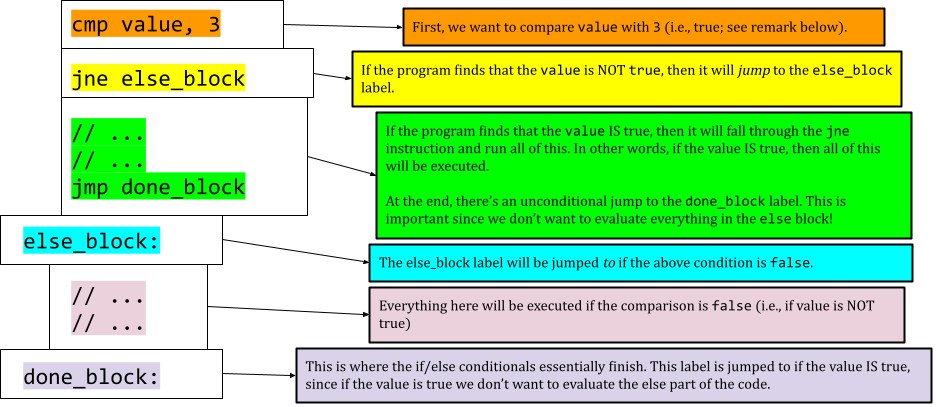
\includegraphics[scale=0.5]{../assets/asm_if.png}
\end{center}
\textbf{Remark:} \code{3} is represented as \code{true} (the binary representation of \code{3} is \code{11}; notice how the tag bit is \code{1}).

\subsubsection{Duplicate Labels}

All \code{if}-expressions will follow the same pattern\footnote{Maybe not the exact pattern, but the same behavior}. However, if we just use this same exact template, we'll end up with multiple duplicate label declarations. In other words, we might end up with something like 
\begin{verbatim}
    cmp value 3
    jne else_block 
    // ... 
    jmp done_block 
else_block:
    // ... 
done_block:
    // ...
    cmp value 3
    jne else_block 
    // ... 
    jmp done_block 
else_block:
    // ... 
done_block:\end{verbatim}
This code would fail to run since there are, for example, duplicate \code{done\_block} label declarations. So, we need to create a unique label whenever we do declare a label. Let's declare a function that does just this: 
\begin{verbatim}
    fn new_label(l: &mut i32, s: &str) -> String {
        let current = *l;
        *l += 1;
        format!("{s}_{current}")
    }\end{verbatim}
At a high level, \code{new\_label} takes in a mutable reference to an integer and a string, and creates a label using those inputs. The integer is incremented -- this is important since this guarantees that every label created from this function will be unique.

\subsubsection{The Equals Comparison Operator}
How do we check if two expressions are equal? The process is relatively similar to adding two expressions. The only difference is at the end, when instead of actually \emph{adding} the values, we put either 3 (\code{true}) or 1 (\code{false}) into \code{rax}.

\bigskip 

The way we do this (putting either \code{3} or \code{1} into \code{rax}) is literally just another \code{if}-statement! At a high level, this might look like: 
\begin{verbatim}
    if rax == [rsp - stack_offset] {
        rax = 3
    } else {
        rax = 1
    }\end{verbatim}
So, compilation might look something like this: 
\begin{verbatim}
    match e {
        Expr::Eq(a, b) => {
            let a_instr = compile_expr(a, si, env, counter);
            let b_instr = compile_expr(b, si + 1, env, counter);
            let else_label = new_label(counter, "ifelse");
            let end_label = new_label(counter, "ifend");
            let stack_offset = si * 8;

            format!("
            {a_instr}
            mov [rsp - {stack_offset}], rax
            {b_instr}
            cmp rax, [rsp - {stack_offset}]
            jne {else_label}
              mov rax, 3
              jmp {end_label}
            {else_label}:
              mov rax, 1
            {end_label}:
            ")
        }
        ...
    }\end{verbatim}

\subsubsection{\code{if}-Expressions}
With everything in mind, our final implementation of \code{if}-expressions will look something like the below.
\begin{verbatim}
    match e {
        Expr::If(cond, thn, els) => {
            let end_label = new_label(counter, "ifend");
            let else_label = new_label(counter, "ifelse");
            let cond_instrs = compile_expr(cond, si, env, counter);
            let thn_instrs = compile_expr(thn, si, env, counter);
            let els_instrs = compile_expr(els, si, env, counter);
            format!(
                "
               {cond_instrs}
               cmp rax, 3
               jne {else_label}
                 {thn_instrs}
                 jmp {end_label}
               {else_label}:
                 {els_instrs}
               {end_label}:"
            )
        }
        ... 
    }\end{verbatim}
At a high level, 
\begin{itemize}
    \item First, we should evaluate the conditional part of the \code{if}-statement. We should\footnote{We'll talk more about type validation later.} end up with a boolean value in \code{rax}. 
    \item With the boolean value in \code{rax}, we can determine which code (either the ``then'' or ``else'' blocks) to run. 
\end{itemize}

\end{document}